\documentclass[11pt, letterpaper]{article}

\input{preamble}
\input{commands}
\usepackage[backend=biber, style=authoryear]{biblatex}
\usepackage{subcaption}
\addbibresource{references.bib}

% ==========================================
% DOCUMENT START
% ==========================================
\begin{document}

\begin{titlepage}
   \begingroup 
    \centering
    \vspace*{2.5cm}
    
    % Elegant Horizontal Rule
    \rule{\textwidth}{1.5pt}\vspace{0.5cm}
    
    {\huge \bfseries \scshape On Par Golf} \\
    \vspace{0.3cm}
    {\Large \itshape Leveraging Gaussian Process Regression for Perfect Golf} % Optional Subtitle
    
    \vspace{0.5cm}
    \rule{\textwidth}{1.5pt}
    
    \vspace{3cm}
   \endgroup 
    
    \section*{Abstract}
    \noindent
       Golf is fundamentally a problem of sequential decision-making under uncertainty, where a surplus of strategic options often obscure the optimal path to the hole. This project presents a data-driven framework that quantifies player-specific optimal strategies by fusing historical course data encoding local difficulties with player-specific tendencies using Gaussian Process Regression. Moving beyond traditional biomechanical analysis, we model the golf course as a continuous risk surface, learning the ``scoring potential'' of every location based on course geometry, historical data, and the player's shot tendencies. The primary output of this framework is a tangible, actionable strategy: the collection of optimal club and aimpoint recommendations for any coordinate on a given hole, under either a conservative (expected-strokes-minimising) or aggressive (birdie-probability-maximising) objective. Our model requires \fillin simulated outcomes per decision location to reach over 80\% convergence on overall strategy; the residual instability detected by our model reflects genuine near-ties in the risk surface instead of simulation noise. Independent of prior empirical strokes-gained-based analyses, our model recovers the finding that distance gains dominate dispersion improvements when looking at expected score. Ultimately our framework replaces guesswork with computation, identifying the set of club and aimpoint combinations that statistically optimise a player's outcome from any location on the course.
    \vfill
    \today
\end{titlepage}

% -------------------------------------------------------
% MAIN BODY
% -------------------------------------------------------
\newpage
\setcounter{page}{1} % Reset count so Introduction is Page 1

\section{Introduction and Research Question / Background \& significance}
\label{sec: Intro}

Golf is a deceptively simple sport: get the ball into the hole in the fewest number of strokes possible. Upon closer inspection, however, this objective is marred by complexity. Over the course of a round, a player faces 18 holes made up of differing lengths and topographies, riddled with obstacles: water hazards, sand traps, and out-of-bounds limits with associated penalties. Consequently, no player will ever face the exact same shot twice.

Traditionally, golf performance has been viewed through a biomechanical lens. Striking a ball smaller than 2 inches in diameter with a club head moving at 135 mph toward a distant target is no small feat. Consequently, the status quo is an obsession with technical perfection: the pursuit of optimising the biomechanical motion of the swing to maximise energy transfer and consistency. This fixation is evidenced by the proliferation of AI-driven swing analysis tools such as Sportsbox.AI, GolfFix, and Sparrow Golf. \newcite

Said focus on mechanics is not statistically unfounded. In 2014, Mark Broadie provided statistical evidence that driving distance is a key factor and strong predictor of success on the PGA Tour\footnote{PGA Tour: Professional Golf Association, US-based organisation running the main professional golf circuit.} - often more important than accuracy or putting (which had long been hypothesised to be the most important part of the golf game) \parencite{Broadie_2014a}. PGA Tour professionals who drive their ball 20 yards further than their peers typically save about 0.75 strokes per round, translating to a substantial 3 strokes over a four-day tournament. The primary way to hit the ball further is to maximise ``smash factor'', which implies optimising technique. We return to this claim in Section \ref{subsec: genObs}, where our simulation-based framework independently recovers said result through an entirely different mechanism. 

While mechanical questions are valid, they give rise to critical counter-questions: is there a way to optimise the tools we already have? How can we improve our scores independently of ``getting better'' at swinging a club? 

Ideally, the tour professional's swing is mechanically optimised, yet scoring divergences persist between the top 50 players, consistent winners, and the rest. For the recreational amateur, while technique has a large margin for improvement, meaningful mechanical changes require time, patience, and financial investment. Both professionals and amateurs can benefit from taking a different approach.

Golf is not solely about physical execution; it is a problem of complex sequential decision-making under uncertainty. There are  millions of sequences of different shots that can get the ball into the bottom of the hole. A player faces the course with up to 14 clubs and the possibility of hitting dozens of shot types. Such flexibility creates a ``paradox of choice''; a psychological hurdle where an abundance of options obscures the best path forward \parencite{schwartz2015paradox} and where decision theory and statistics become relevant. By treating every shot as a mathematical calculation of risk versus reward, we can determine the optimal path to the hole. 


Any such calculation, however, is only as good as the data used to learn it. Individual players and small golf programs will rarely have access to a ShotLink-scale \footnote{ShotLink is the PGA TOUR's official data collection system, capturing high-precision spatial metrics for every stroke played during professional tournaments. Using 3-dimensional course mapping, radar, and laser tracking technology, ShotLink records detailed variables including shot distance, exact ball coordinates, lie condition, and distance to the target hole.} \newcite, player-specific outcome datasets covering every position on every hole they play. What is available instead is the opposite: generic, sparse, course-level data reflecting how golfers in general have scored from a given position over time, but carrying no information about any individual player's own skill, tendencies, or intent. Additionally, a player can recover their own shot tendencies quite precisely --- manually, or with a launch monitor such as Trackman \newcite --- but this only characterises the dispersion of shots hit from a single origin along a single target line; it says nothing about how difficult any particular landing spot on the course actually is to score from. Seldom is course-level or player-specific data useful in isolation: the course-level data has no notion of the player, and the player-level data has no notion of the course. Building a player-accurate, spatially complete risk surface requires fusing both datasets, which is the central methodological problem this paper addresses.

To this end, our paper proposes a data-driven framework allowing an individual player to quantify their optimal strategy on a given golf course by leveraging both course- and player-specific data. We 
approach the decision theory scenario through a Bayesian lens, using prior performance data to help inform future strategic choices. By implementing a multi-fidelity Gaussian Process Regression framework, we construct continuous predictive surfaces that evaluate the ``scoring potential'' of all possible landing zones on a golf course, adjoining historical outcomes with player-specific shot data. Our model allows us to mathematically define the player's objective through different ``loss functions'' --- whether minimising the expected number of strokes to hole out for consistent play or maximising the raw probability of a birdie when the need to exhibit a more aggressive play style arises. Ultimately, our framework replaces guesswork with calculation, identifying the specific club and aimpoint combinations that statistically optimise a player's outcome from any location on the course.


The remainder of this paper is organised as follows: Section~\ref{sec:Background} places our work within the broader context of sports analytics and reviews existing literature. Section~\ref{sec:Data} describes the data we used, and Section~\ref{sec:Modeling} explores the modeling mechanisms employed alongside an evaluation of some of the experiments we performed on our modeling engine. Section~\ref{sec:Results} presents the results of our simulations, and Section~\ref{sec:Discussion} discusses the limitations of the current framework alongside potential avenues for future expansion.  Appendix~\ref{sec:Appendix} presents the data generating mechanism we used to supplement our existing data and Appendix~\ref{sec:Appendix2} includes a glossary of relevant terms.

\section{Background and Significance}
\label{sec:Background}

The shift toward objective strategy in sports is not unprecedented. This project draws direct inspiration from SABRmetrics \parencite{albert2010sabermetrics}: the empirical analysis of baseball that uses statistics to evaluate player performance and inform objective, data-driven decisions. Coined by Bill James, this non-traditional statistical investigation famously allowed the Oakland Athletics to remain competitive against teams with much larger budgets by using data to identify and acquire undervalued players \parencite{moneyball_lewis}. Here, we apply the same philosophy to golf: replacing subjective intuition with statistical decision-making.

Historically, golf analysis relied heavily on total score and basic counting stats (fairways hit, putts per round), which often failed to capture the true quality of a shot. This landscape changed with the introduction of Strokes Gained, SG \parencite{Broadie_2014a}. The SG metric redefined performance evaluation by establishing baselines for the expected number of strokes to hole out from any distance and lie on the course. For the first time, players had access to interpretable metrics that could isolate specific strengths and weaknesses in their game relative to the field.

Strokes Gained paved the way for applied course strategy systems, most notably DECADE \parencite{decade_golf}. DECADE is a proprietary course-management system built largely on generalised SG estimates, allowing players to make informed decisions grounded in statistical insight rather than emotion. The efficacy of such systems is well-documented; for instance, Will Zalatoris rapidly ascended from a World Amateur Golf Ranking (WAGR) of 3,000+ to the top 3 in under three months after adopting the DECADE pedagogy \parencite{decade_golf}.

The application of statistics to golf strategy is still an evolving field. Previous work has primarily focussed on three distinct methodologies: Markov Decision Processes (MDPs), neural network classification, and reinforcement learning. While these methods provide a solid foundation for objective decision making, they each exhibit limitations that our project seeks to address.


\textcite{sugawara_skill-based_2013} applied Q-learning within a MDP framework to minimise expected score, and show that optimal strategy is highly skill-dependent. Their green modeling, however, ignores green slope entirely, computing expected putts from distance alone, optimising strategy for a two-dimensional idealisation of a three-dimensional game, while not utilising course specific data. 

\textcite{stauffer_golf_2025} show that golf strategy can be solved exactly as a stochastic shortest path problem via value iteration on Trackman-derived player profiles, without heuristic approximation. Their model treats greens as flat surfaces and assumes that historical shots are always aimed at the pin, a critical choice that we aim to address in our modeling framework. They also impose risk-neutral decision-making throughout their modeling mechanism overall producing simulated strategies that are riskier than those observed in professional performance. 

\textcite{khazaeli_golf_2024} trained multi-level neural network classifiers on a NCAA Division I dataset augmented via Monte Carlo simulation, predicting approach-shot outcome zones on 27 features, including distance, terrain, and atmospheric conditions such as wind strength and lie. The study is limited to approach shots, relies heavily on synthetic augmentation, and functions primarily as a classification tool used to predict outcome zones instead of providing strategy optimisation.

The limitations of prior work point to a common root cause rather than three unrelated shortcomings. MDP and reinforcement-learning formulations \parencite{sugawara_skill-based_2013, stauffer_golf_2025} rely on course geometry or player profiles in isolation rather than binding the two together for a specific player on a specific hole; neural-network classifiers
\parencite{khazaeli_golf_2024} are trained on a fixed population's data and cannot be adjusted to an individual player's own tendencies without retraining. None of work described here treats course-specific difficulty and player-specific skill as data to be actively combined for the decision at hand.

Whether through direct comparison of a player's shot profile against a digitised course (Sections~\ref{subsec:par3}--\ref{subsec: par4b}) or through the explicit multi-fidelity fusion of location-specific course
outcomes with said player-specific data(Section~\ref{subsec: strategicBlanket}), every risk surface in the GPR framework is built by bringing course-specific information and player-specific data together. The model moves past the generalised, one-size-fits-all
estimates of commercial systems like DECADE \parencite{decade_golf} and produces 
recommendations grounded on both the difficulties of a given course and a player's shot patterns.

\section{Data}
\label{sec:Data}

In order to understand the data inputs that we used when modeling the optimal golf strategy, it is valuable to distinguish between the two data fidelities our model implements: a high-fidelity set of historic course-level data, and low-fidelity, player-specific data. The type of data needed for our model exists within proprietary software. Without access to such data, we utilise a proxy dataset to develop a proof of context. Our model is agnostic to the source of its dataset; it requires three specific layers of information to work: course geometry for lie classification, location-specific outcome data, and player shot distribution data.

\subsection{The two data fidelities} 
\label{ref:idealData}

Our model draws on two kinds of data, differing in reliability. High-fidelity data, $\mathcal{D}_H$, consists of real, location-specific historical outcomes: observations of how many strokes it actually took real players to hole out on a particular hole from a given spot. Such data is sparse and expensive to obtain, since it requires data point recorded at precise locations, but it is ground truth of past outcomes wherever it exists. The low-fidelity data, $\mathcal{D}_L$, consists of simulated \altw{expected} outcomes: dense and cheap to generate from a player's own shot-dispersion profile via Monte Carlo
methods (Section~\ref{subsec: playerSim}). We always simulate $\mathcal{D}_L$ since no individual golfer will ever recover hundreds of recorded strokes-to-hole-out observations from every position on a hole. It follows that $\mathcal{D}_L$ will only ever be as accurate as the underlying processes used to simulate the player's outcomes.

The two kinds of data play out differently across the three regions of the course that our framework models. Despite being 
synthetic in this paper, (Section~\ref{subsec: greendata}), data used to model green and near-green outcomes are considered $\mathcal{D}_H$, as green differences and difficulties for a given pin are uniform across different player levels and don't need to be player-specific to accurately convey difficulty.
It is for the long game --- the intermediate landing zones between tee and green on par 4s and potentially par 5s --- that both fidelities are actually constructed and combined: a dense $\mathcal{D}_L$, built purely from simulation (Section~\ref{subsec: strategicBlanket}), is fused against a sparse, real-outcome $\mathcal{D}_H$ (Appendix~\ref{app: long-game data}), via the multi-fidelity model of Section~\ref{subsec: strategicBlanket}.

In a fully realised application, such as one using the PGA Tour's ShotLink system and a player's shot history, our model would consume the following:
\begin{enumerate}
    \item \textbf{Location-Specific Outcome Data:} A large repository of historical shots describing how many shots it took players to complete the hole from different locations. From the origin (starting location) of any recorded shot, $\origin$, a coordinate in the Cartesian plane, we observe the discrete outcomes of how many shots it took players to hole out to the corresponding hole. The number of shots intrinsically encodes the underlying ``difficulty'' of said ``random'' spot: locations with the same Euclidean distance to the pin where the average strokes to hole out are higher than others are inherently ``harder'' (see Figure ~\ref{fig:shot_data}).
    \item \textbf{Course Geometry for Lie Classification:} A high resolution, bird's-eye view vector map of the hole (where the tee is at $(0,0)$). This allows our model to embed course geometry into the model by instantly classifying any coordinate $(x_1,x_2)$ as a specific lie type (i.e., Fairway, Rough, Deep Rough, or Bunker), triggering the appropriate modeling and decision logic.

\begin{figure}[h]
    \centering
    \includegraphics[width=.8\linewidth, height = .2\linewidth]{images/ShotData.png}
    \caption{\textbf{Visualisation of Location-Specific Outcome Data.} 
    The figure illustrates the recorded paths of different players (distinguished by colour) on the digitised hole. The numeric labels at each coordinate indicate the observed number of strokes they took to hole out from that specific location. The discrete observations with coordinates serve as the raw input for encoding the underlying difficulty of every position on the course.}
    \label{fig:shot_data}
    \nts{annotate the tee, change the red cross for something else}
\end{figure}
    \item \textbf{Player Shot Distribution Data} A library of ``stock shots'' labeled by the player. Whether recorded on a launch monitor (e.g., Trackman, GCQuad) or manually logged, the dataset would consist of the landing coordinates $\landing$ generated by hitting shots from  $\origin$ aiming down a set target line (where the lateral offset is zero) for every repeatable shot in a player's repertoire\footnote{In addition to the 14 clubs they usually carry in a bag, competitors usually identify different kinds of shots they can hit with their clubs. These shot-types tend to impact the ball's flight affecting factors such as the ball's lateral curve, apex height, or total carry distance. While most players recognise and play standard full swing shots, a player may choose to name additional shots in distinct ways (e.g., a player may name a specific shot an L-shot, while another may name it a 3/4 swing). Trackman allows the player to individually record and save shots under different names, which are then modelled in such a way that the output of our framework includes recommendations implementing such labelled shots.}. 
    
    Ideally, we would have labelled data from different starting lies such as rough or fairway bunkers, accounting for the increased dispersion and variance that results from hitting off of different surfaces. More concretely, the player's shot library would contain observations encoding the tuple $\left(\origin, \;\landing,\; Lie\right)$ for every specific labelled $Shot$ type. From data in said format, we derive enough information to fully characterise the conditional landing distribution $P\left(\landing\;|\;Shot,\; \origin,\; Lie\right)$.
\end{enumerate}

\nts{Maybe i want 2 images side to side. 1 historical data used to train of par 4, the simulated grid of ESHO on the par 4, i.e. lower fidelity data and higher fidelity data  (will be referenced in the future too)
}
\begin{figure}[h]
    \centering
    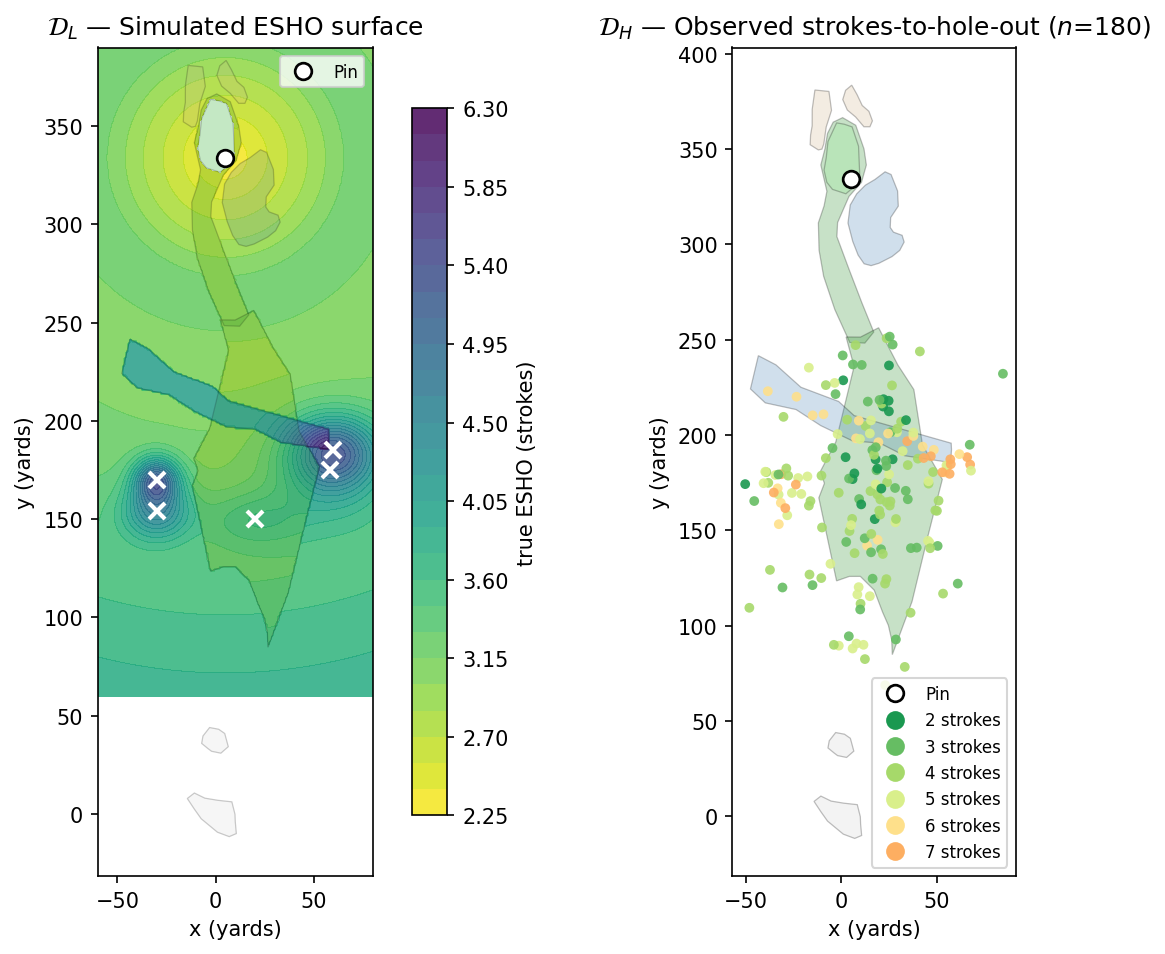
\includegraphics[width=0.8\linewidth]{images/dl_vs_dh_curated.png}
    \caption{$\mathcal{D}_L$ (simulated ESHO surface) vs. $\mathcal{D}_H$ (sparse observed strokes-to-hole-out proxy).}
    \label{fig:dl_vs_dh}
\end{figure}

\subsection{Data Implemented in this Study}

To demonstrate the viability of our framework, we developed and implemented a robust proxy dataset (defined in Appendix \ref{sec:Appendix}) that provides an appropriate substitute for the three core data layers required by the model. We successfully digitised a real golf course using satellite imagery and vector mapping tools, achieving the high fidelity of the ideal data for our course geometry. In the absence of proprietary PGA Tour ShotLink data, we built a data-generating mechanism to emulate location-specific strokes-to-hole-out outcomes, supplemented by empirical estimates. Finally, we established a representative LPGA\footnote{LPGA: Ladies Professional Golf Association} Tour player profile using publicly available launch monitor statistics to model the player's shot distribution data.

\subsubsection{Course Geometry}
We digitised hole 9 of Mountain Meadows Golf Course in California, a par 3 chosen for its rich interaction of obstacles such as bunkers and water hazards near the green. The course layout was scraped using OpenStreetMap \parencite{openstreetmap}, and refined in QGIS \parencite{qgis} to create accurate vector polygons compatible with the \texttt{Shapely} \parencite{shapely} library in Python. To test chained-decision-making (par 4 strategy), we manually generated a hypothetical extension of hole 9 adding a secondary water hazard to increase strategic complexity. 

\subsubsection{Emulating Location-Specific Outcome Data}
\label{subsec: greendata}
\begin{itemize}
    \item \textbf{On the green:} We generated a dense sample of synthetic putting outcomes for our digitised green taking into consideration slope and distance in a three dimensional setting (see Appendix \ref{app: green-surface data}). The data generated simulates the ``ideal'' data,  $\mathcal{D}_H$, described in subsection \ref{ref:idealData}, providing a count of the strokes to hole out for hundreds of points on the putting surface. The proxy data is displayed  in Figure \ref{fig:Putts}.
    \begin{figure}[h]
        \centering
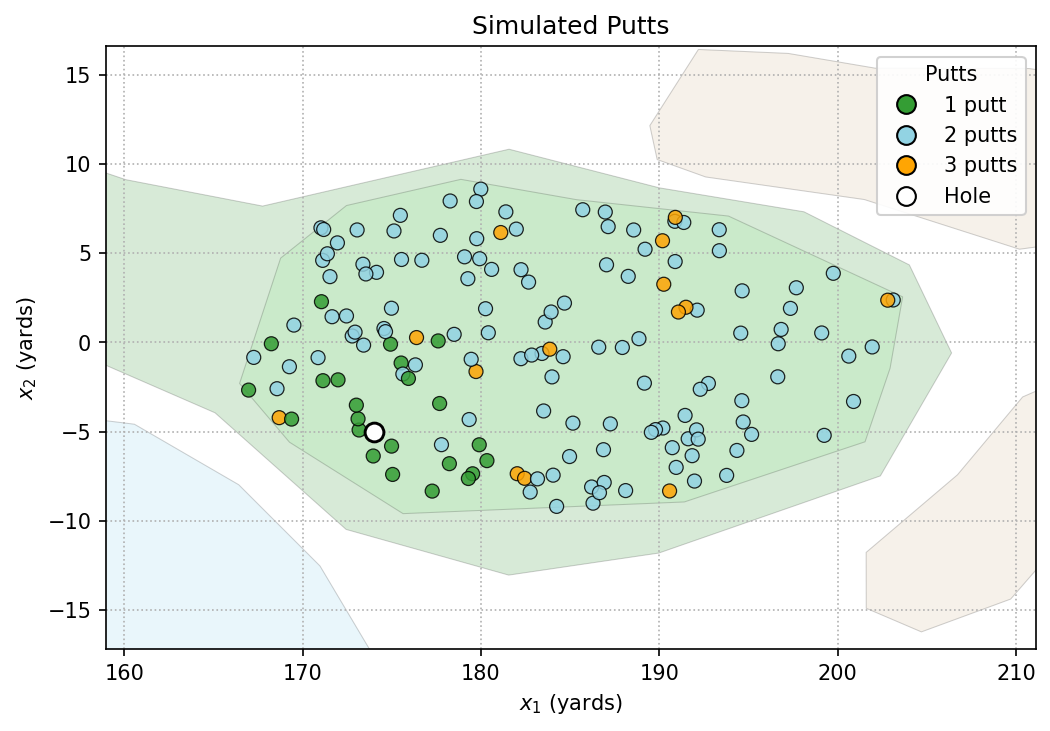
\includegraphics[width=0.4\linewidth]{images/sampledPutts.png}
        \caption{Synthetic putting dispersion pattern on our green.
The figure shows the modelled distribution of putt outcomes relative to a fixed pin location (black dot). The position of each point represents a starting position of a sequence of putts, and the colours indicate the number of strokes it took to hole the ball from said position:  green for one-putt, blue for two-putt, orange for three-putt, and red for four-putt results.
\nts{Make hole more distinguishable}}
        \label{fig:Putts}
    \end{figure}

    \item \textbf{Off/Around the Green:} The high-fidelity data that would ideally exist here is not available to
us. We therefore fall back on Mark Broadie's published
``strokes to hole out'' estimates by distance and lie (derived from PGA Tour ShotLink data
from 2003-2012, published in Every Shot Counts \parencite{Broadie_2014a}), which can also be
found in Appendix~\ref{app: short-game data}. This is a flat, non-spatial baseline rather than
a generated $\mathcal{D}_H$-style dataset, but given an appropriate dataset would instead be modelled in
conjunction with the green data as high-fidelity data.


\change

\nts{I probably want to say something like, we didn't bother generate short game data... which would be ideal, and encode more location specific information, we rely on empirical estimates but given the appropriate $\mathcal{D}_H$ data, we would fit the GPR on both the  green data and around the green uniformly, it would just give us a larger area to regress or evaluate on. }
It is worth noting that while we utilise LPGA Tour data for full-swing dispersion (see
Section~\ref{sec: playerShotUsed}), we rely on PGA Tour baselines for short game outcomes due
to the availability of their empirical estimates. We posit that the relative difficulty of
short-game scenarios (the penalty of a bunker shot or a short-sided chip) remains comparable
across professional tours. Moreover, as this framework is data-agnostic, the presence of
mixed-source data does not undermine the validity of the optimisation logic.

\item \textbf{Long Game:} We use \textit{long game} to describe any non-putting shot attempts at  distance greater than 50 yards from the hole. When simulating these shots, we uniquely construct and fuse both data-fidelities. The low-fidelity layer, $\mathcal{D}_L$, is built purely via monte-carlo simulation: we simulate shots from each intermediate grid point to the pin and evaluate them
via the function $AG(\out)$ which aims to establish the shots to hole out from the landing positions, exactly as described later on in Section~\ref{subsec: strategicBlanket}. The high-fidelity layer, $\mathcal{D}_H$, is a sparse, proxy real-outcome dataset generated to
emulate the kind of location-specific historical strokes-to-hole-out observations, at long game coordinates in the rough, fairway, sand, and near water hazards (Appendix~\ref{app: long-game data}). The high-fidelity and low-fidelity datasets are fused via the multi-fidelity model in Section~\ref{subsec: strategicBlanket}, updating the purely-simulated grid against real outcomes before it is used to value the tee shot.
\nts{need to define more accurately the distances this captures}

\end{itemize}

\subsubsection{Player Shot Distribution Data}
\label{sec: playerShotUsed}

We utilised a proxy shot distribution data set based on publicly available Trackman launch monitor statistics for a representative ``average'' LPGA tour player \newcite. The library encompassed 13 standard clubs from $60^\circ$ wedge to a Driver (ranging approximately $66$ to $250$ yards), plus several partial wedges for shorter distances. For each of the $20$ shot-types recorded in this proxy player's repertoire, the dataset contains 30 recorded landing coordinates, totalling 600 observations. We assume all of the shots are hit off the fairway (or a tee in the case of a Driver). The coordinates generated based off LPGA data were generated from shots hit along a single target line (zero lateral offset), providing the necessary dispersion characteristics to model the player's skill profile (see Figure \ref{fig:dispersion}).

\label{img: dispersions}
\begin{figure}[h]
    \centering
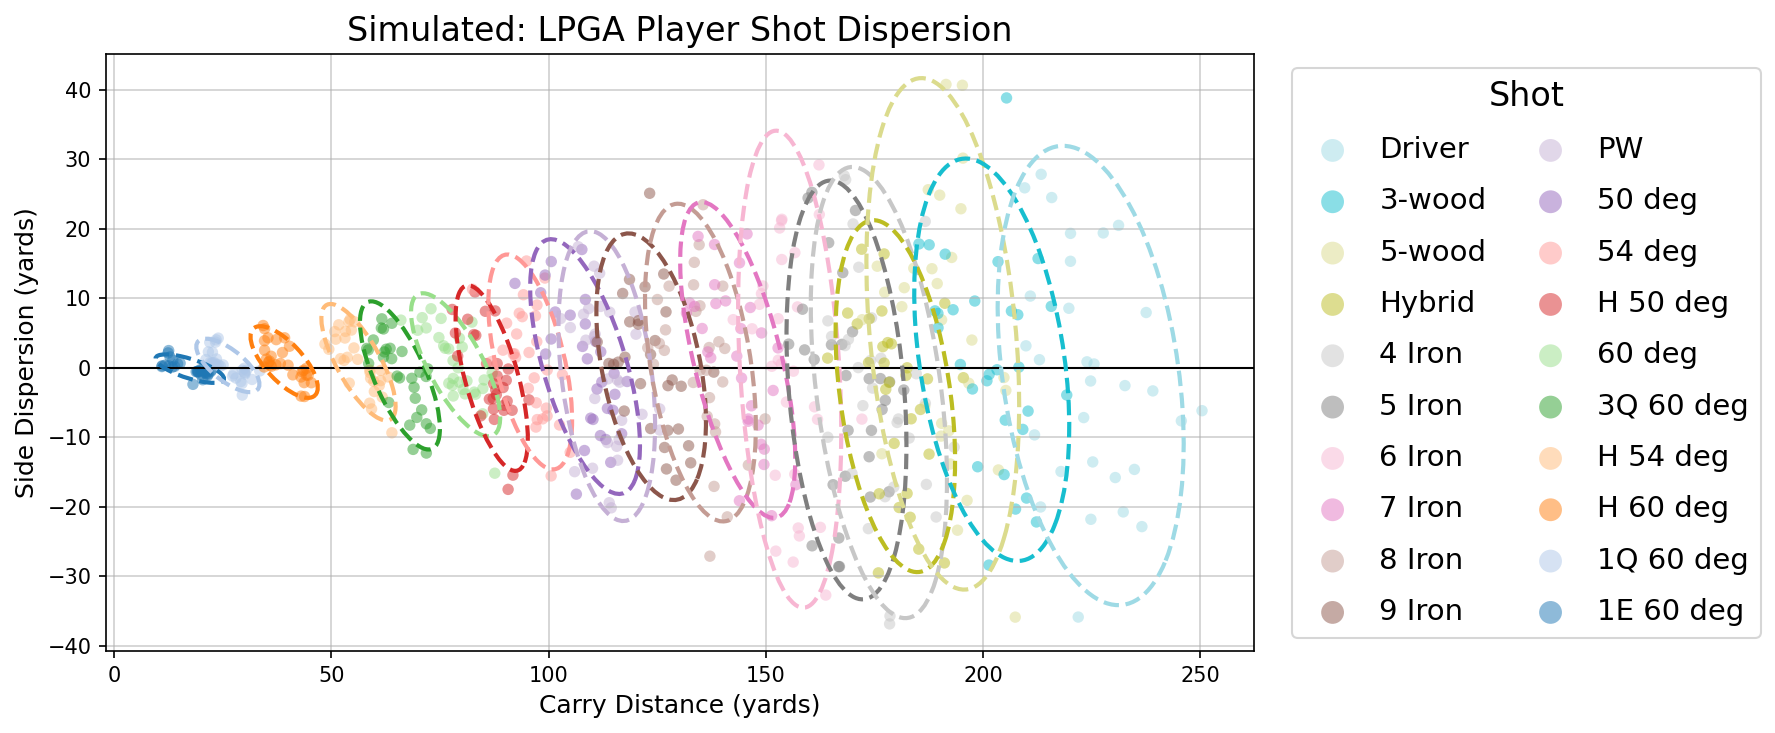
\includegraphics[width=0.6\linewidth]{images/LPGAShots.png}
    \caption{\textbf{Stochastic Modeling of Player Dispersion.} 
    Visualisation of the proxy LPGA player's shot library. The covariance ellipses represent the $95\%$ confidence region for landing coordinates across varying club types. Note the heteroscedasticity of the data, where dispersion ($\Sigma_s$) increases non-linearly with distance, a critical factor for the GPR model's risk assessment.}
    \label{fig:dispersion}
\end{figure}
\nts{keep but maybe i want to add another one for different sensitivities later on. Point out tilt in description. Increase size of legend (side by side.}

\section{Modeling and Methods}
\label{sec:Modeling}

\subsection{Our Mathematical Framework: Decision Theory}

Ben Hogan, who was widely regarded as one of the greatest ball strikers in golf history, famously stated that even on a great day, he would hit at most three  truly great shots in a round \parencite{Jenkins_1998}. The inherent imperfection in performance means golf fundamentally poses a problem of decision-making under uncertainty.

In statistical decision theory, we usually seek a decision rule $\delta$ that minimises a specific loss function $\mathcal{L}$. In the context of a golf shot, our decision rule is a tuple $\delta = (s, \aimpoint)$, where $s$ represents the discrete choice of club/shot type and $\aimpoint \in [-20^\circ, 20^\circ]$ \fillin represents the continuous choice of the aimpoint's lateral offset from the pin (where negative values denote aiming left of the pin, and positive values denote aiming right). The outcome of the decision, which is the actual landing coordinate of the ball, is denoted by the random vector $\Out \in \mathbb{R}^2$. Given that human performance is imperfect and that there are ever-changing variables, the landing is stochastic, drawn from a probability density function conditioned on the player's decision: $\Out \sim f(\out | s, \aimpoint) $. We denote the realised outcome of this variable as $\out^l = \landing$.

    \nts{I HAVE A FIX for the degree issue. I should just do it with yards directly.}

The objective of our model is to find the decision $\delta$ minimising the expected cost of a shot. The loss function, $\mathcal{L}(\Out)$, measures the cost (or penalty, in strokes) incurred when the ball lands at coordinate $\Out$. In a deterministic scenario where the outcome $\Out$ is certain, we would simply minimise the known loss $\mathcal{L}(\Out)$. However, we are operating in an imperfect and therefore stochastic paradigm, where the outcome is governed by the probability density function $f(\out | \delta)$. The nature of golf requires minimising the risk, $R(\delta)$, defined as the expected loss over the player's shot outcome distribution:

$$R(\delta) = \mathbb{E}_{\Out|\delta}[\mathcal{L}(\Out)] = \int_{\mathbb{R}^2}\mathcal{L}(\out)f(\out | \delta)d\out$$

The choice of loss function, $\mathcal{L}$, critically shapes the optimal strategy. In standard statistical modeling, we often select symmetric loss functions. For example, the symmetric Squared Error Loss, $\mathcal{L}^*(P, \hat{P}) = (P - \hat{P})^2 $, assumes that an error of magnitude $\epsilon$ is equally detrimental, regardless of direction. 

However, golf, like many real-world scenarios often presents asymmetric loss landscapes. Consider civil engineers designing bridges: building a bridge a foot too long is a minor inefficiency and cost when compared to the catastrophic failure of building it a foot too short. Golf exhibits similar non-linearities. A shot missing a few yards to the left might rest safely in a spot fractionally less optimal than the ``perfect'' spot, whereas one missing a few yards right could plunge into a water hazard, incurring a fixed penalty stroke and a positional disadvantage.

While we can conceptually define different loss scenarios, the resulting risk function $R(\delta)$ remains an elusive unknown surface over the two dimensional domain of a golf course. We don't have an analytical formula that outputs the expected loss for any given coordinate $\out^l$: we only have sparse, noisy observations of shots and scores. To perform any sort of optimisation, we need to first learn the associated risk surface for a specific hole (no two holes are exactly alike!). The definition of such a surface requires a statistical method capable of taking in scattered data to predict a continuous landscape of expected strokes to hole out (ESHO), a task for which we can leverage Gaussian Process Regression (GPR). 

In this project, we define two distinct risk landscapes that our GPR models can learn, corresponding to different player objectives.


\begin{enumerate}
    \item \textit{Minimising Expected Strokes to Hole Out.} Here, our loss function, $\mathcal{L}_\mu$,  is the count of strokes to hole out from any given landing position. $ \out \in \mathbb{R}^2$, and outputs the expected number of strokes.

    The function is defined as: $\mathcal{L}_{\mu}:\; \mathbb{R}^2 \to \mathbb{Z}^+$
    $$\mathcal{L}_\mu(\out^l)= \text{Strokes to hole out from }\out^l$$
    The associated risk, $R_{\mu}$, is the expectation of the aforementioned loss given a specific decision $\delta$. The risk function domain is consistent with the decision rule:  $R_{\mu}:\; \mathcal{S} \times [-20^\circ, 20 ^\circ]\to \mathbb{R}$, where, $\mathcal{S}$ is the discrete set of shot types a player chooses from.

    $$R_{\mu}(\delta) = \mathbb{E}[\mathcal{L}_\mu(\Out) | \delta]$$
    
    By minimising $R_{\mu} (\delta)$ we identify decisions where the average outcome (Expected Strokes to Hole Out) is the lowest. We naturally account for asymmetric hazards because the penalised observations fundamentally skew the local mean upwards. The actual optimisation mechanism is explored in Sections \ref{subsec:par3} and \ref{subsec: par4}.

    \item \textit{Maximising Birdie Probability.} 
    
    Additionally, we employ a utility-based loss function, where ``success'' and, by complementation, ``loss'', is binary. The loss is defined based on whether the expected score from the landing spot $\out$ fails to achieve the birdie target. 

    The loss function $\mathcal{L}_B$, maps the landing position $\out$ to a binary outcome, $\mathcal{L}_B: \mathbb{R}^2 \to \{0,1\}$.

    $$\mathcal{L}_B(\mathbf{x}) = \begin{cases} 0 & \text{if } \text{score from } \mathbf{x} < \text{Par Score, (i.e., Birdie or better)} \\ 1 & \text{if } \text{score from } \mathbf{x} \ge \text{Par Score (i.e., Par or worse)} \end{cases}$$

    The associated risk, $R_B$, is the probability of failure (not making a birdie or better), $R_B: (\mathcal{S} \;\times \;[20^\circ, -20^\circ]) \to [0,1]$. Since the loss is binary, the expectation is equivalent to the probability of the loss occurring: 
    
    $$R_B(\delta) = \mathbb{E}[\mathcal{L}_B(\Out)|\delta] = \mathbb{P}\left(\text{Strokes to Hole Out from } \Out \geq \text{Par Score} | \delta \right)$$
    
    The minimisation of $R_B(\delta)$ value reflects the ``must-score'' scenarios where the magnitude of a miss is irrelevant (a par is as useless as a triple bogey). 

     The actual optimisation mechanism is explored in Section \ref{subsec: par4b}.
\end{enumerate}


\subsection{Our Modeling Engine: Gaussian Process Regression}

Gaussian Processes are distributions of functions where any finite subset of points follows a multivariate Gaussian distribution. As expected, they are fully specified by their mean function $m(\out) = \mathbb{E}(f(\out))$  and covariance kernel $k(\out,\out') = \mathbb{E}[(f(\out)-m(\out))(f(\out')-m(\out'))]$:

\begin{equation}
    f(\out) \sim \mathcal{GP}(m(\out), k(\out,\out'))
\end{equation}

In our context, $\out$ represents the spatial coordinates on the hole ($\out = \coord$), and $f(\out)$ represents the latent scoring potential of any given position (e.g., $f$ encodes the number of strokes to hole out from a given position).

\subsubsection{Covariance Kernels}
The heart of Gaussian Processes are the kernel functions, $k(\out,\out')$, which encode our prior assumptions about the structure of the data. To capture the aforementioned spatial coherence of a golf course, we use the Radial Basis Function (RBF) kernel:

$$k(\out,\out') = \gamma^2\exp\left(-\frac{||\out-\out'||^2}{2l^2}\right)$$

where the hyperparameters dictate the surface's behaviour and flexibility. The length-scale, $l$, controls the flexibility of our functions, controlling smoothness by dictating how quickly scoring difficulty changes over distance. Smaller values of $l$ drive correlations to $0$, allowing functions to exhibit ``wilder'' or more jagged behaviour, while also relaxing the width of confidence bounds. The signal variance, $\gamma^2$, on the other hand, controls the vertical amplitude of the function we are trying to estimate.

We model our observed data $\mathbf{y}$ (i.e., actual strokes taken from a spot) as the latent function with Gaussian noise: $y = f(\Out) + \epsilon$, where $\epsilon \sim \mathcal{N}(0, \sigma^2)$. $\sigma^2$ captures irreducible shot-level noise at a given location.

Given a set of $n$ observed training points $\Out$ and outcomes $\mathbf{y}$, and a new test location $\out_*$ (a new spot we want to evaluate), the joint distribution of the observed data and the unobserved latent function value $f(\out_*)  \equiv f_*$ is given by:

\begin{align*}
    \begin{bmatrix}
        \mathbf{y}\\
        f_*
    \end{bmatrix} \sim 
    \mathcal{N}\left (\begin{bmatrix}
        k(\Out,\Out) + \sigma^2I & k(\Out,\out_*) \\
        k(\out_*, \Out) & k(\out_*, \out_*)
    \end{bmatrix}\right)
\end{align*}
 By conditioning on the observed $\mathbf{y}$, we derive the posterior predictive distribution for the risk at our new location $\out_*$:

\[f_* |\Out, \mathbf{y}, \out_* \sim \mathcal{N}\left(\bar f_*, \text{Var}(f_* | \Out, \mathbf{y}, \out_*\right)\]

Where the posterior mean $\bar f_*$, at a specific location, provides our point estimate for optimal strategy and the posterior variance quantifies our uncertainty.

Nothing about this posterior depends on where the training pairs $(\mathbf{X}, \mathbf{y})$ came from --- only on their locations and observed values. The flexibility of Gaussian Processes allows us to reuse the same machinery in different ways throughout the paper: fit directly to a single data source in some regions of the course where we focus primarily on unfolding the difficulty of the course on its own; and fused across two data sources in other areas where we care to model a player's shot patterns. We introduce each choice where it becomes relevant --- a single-source fit for the green (Section~\ref{subsec:par3}), and a two-source, multi-fidelity fusion for the long game (Section~\ref{subsec: strategicBlanket}).

\subsection{Modeling an Optimal Shot. Par 3s}

\label{subsec:par3}

With our modeling mechanism in place, we can now model the decision-making process for a specific shot. We begin with par 3
holes where players usually try to land on the green in a singular shot expecting to hole out in an additional two putts. It follows that we only model the first shot to the green taking into consideration different shots and aimpoints that may be available. Once on the green, the player rarely uses clubs other than their putter; the slope informs their aimpoint decision, not our model. 

We model the decision taken from a fixed starting coordinate $\origin$, which we treat as the origin $(0,0)$ in the shot's local coordinate system. Our optimisation follows a ``green-to-tee" philosophy: by understanding the value of every landing spot on the green, we can inform the optimal decision from the tee (the choice that precedes it). Such an implementation is viable because the problem exhibits optimal substructure, where the ultimate solution to a problem depends on the optimal solutions to its smaller subproblems. Said characteristic is best known as Bellman's Principle of Optimality \parencite{rosu_bellman}.

\subsubsection{Step 1: Fitting GPR to the Green}
Our strategy builds on the GPR model fitted to the green data leveraging the \texttt{Python} library, \texttt{GPyTorch} \parencite{gardner2021gpytorch}, evaluated at the posterior mean. The fitted Gaussian defines an Expected Strokes to Hole Out (ESHO) surface $f_G: \Omega_{green} \subset \mathbb{R}^2 \to \mathbb{R}$, which outputs the expected number of strokes to hole out (ESHO) from any coordinate on the putting surface. In other words, $f_G$ directly implements our loss function $\mathcal{L}_\mu$ for the putting region.

Because $f_G$ is fit to the unique sample of data specific to hole 9's green and particular pin position, $f_G$ intrinsically accounts for the non-linear difficulties (slope, tiering) that a simple distance-based function would miss.

\begin{figure}[h]
    \centering
    \includegraphics[width=0.35\linewidth]{images/gprGreen.png}
    \caption{\textbf{The Continuous Risk Surface ($f_G$).} 
    Posterior mean predictions of the Gaussian Process Regression model fitted to the green's synthetic putting data. The colour gradient represents the Expected Strokes to Hole Out (ESHO), effectively interpolating the difficulty of unobserved locations based on spatial proximity and topographical slope.}
    \label{fig:green_gpr}
\end{figure}

When a simulated shot from the fairway or tee lands on the green, we compute its ``cost'' by evaluating its scoring potential from its resting position.

If a shot lands on the green, the cost is retrieved directly by evaluating $f_G(\out)$. 

Alternatively, if the shot misses the green, we employ an interpolation function $f_A: \mathbb{R}^+ \times \mathcal{C} \to \mathbb{R}^+$, where $\mathcal{C} = \{F, R, S\}$ represents the set of lie conditions (fairway, rough or sand trap). $f_A$ is a function of lie and distance from the hole that outputs the expected number of strokes to hole out. The function is derived from Broadie's empirical estimates for each lie (See Appendix \ref{app: short-game data}).
\nts{$f_A$ stands for around the green but i don't know if we want a more descriptive name.}

Finally, if a shot lands in a water hazard, we simulate a ``drop'' at the nearest point of relief (drawing a direct line from the ball's starting point, and acting as if that the ball landed at the first intersection with land), incurring a penalty stroke and recursively evaluating the cost from the new position.

Formally, we define a global ``Around the Green'' cost function $AG(\out)$, representing the expected strokes to hole out from any location $\out = \coord$ near or on the green:

\begin{equation}
\label{eq: AG}
    AG(\out) = \begin{cases}
    f_G(\out^l)& \text{if } \out^l \in \Omega_{green} \\
    f_A\left(\out^l, \text{Lie}(\out^l)\right) & \text{if } \out^l \in \Omega_{fairway}\; \cup \Omega_{rough} \; \cup \Omega_{sand}  \\
    1 + AG(\out^{drop}) & \text{if } \out^l \in \Omega_{water}
\end{cases}
\end{equation}

\subsubsection{Step 2: Modeling Player Outcomes}
\label{subsec: playerSim}
In order to evaluate the success of a strategy in approaching the green, we must be able to model and simulate the stochastic nature of a player's ball hitting ability. We achieve this by sampling from a normal distribution fitted to the player shot distribution data described in \ref{ref:idealData}, and then transforming the outcomes based on the chosen aimpoint.

\begin{enumerate}
    \item \textit{Fitting Bivariate Gaussians.} First, we analyse the player's historical shot data to create statistical profiles for each of the available shots $s$. This is done by empirically estimating the two-dimensional centre of data $\mathbf{\hat\mu_s}$ and the covariance matrix $\mathbf{\hat\Sigma_s}$ for the landing coordinates of shots aimed directly at the pin (zero lateral offset) hit with shot $s$ (assuming the player is hitting off the fairway) for . This step ``learns'', for each kind of shot, the player's unique dispersion shape, (see Figure~\ref{img: dispersions}) capturing how their distance control and directional accuracy may vary with different shots, allowing us to generate more data as needed in the following step.
     \item \textit{Monte Carlo Simulation.} We then employ a Monte Carlo simulation to generate a synthetic dataset of potential outcomes. For a selected shot $s$, we draw $N$ random samples from the fitted multivariate normal distribution. 


     \begin{equation}
         \label{eq: shots}
         \Samp^s = \{\samp^{s1}, \samp^{s2}, \ldots, \samp^{sN}\} \text{ where } \samp^{si} \sim \mathcal{N}(\hat\mu_s, \hat\Sigma_s)
     \end{equation}

     Equation \eqref{eq: shots} results in sample of shot outcomes statistically mirroring the player's tendencies,  ensuring a sufficient statistical volume of data to calculate reliable risk estimates even with sparse historical data. 
     As described in Section~\ref{subsec:Convergence}, to attain an overall 80\% convergence and above for our model, we require $N \geq 180$.

     \item \textit{Changing Aimpoints.} Finally, in order to evaluate different strategic aimpoints, we apply a linear transformation to our simulated shots. If a player aims at an angle $\aimpoint$ relative to the pin, we rotate the entire set of simulated outcomes $\Samp^s$ using a standard rotation matrix $\rotation (\aimpoint)$: 

     \begin{align}
         \rotation (\aimpoint) &= \begin{bmatrix}
             \cos \aimpoint & - \sin \aimpoint \\
             \sin \aimpoint & \cos \aimpoint
         \end{bmatrix} \\
         \samp^{si\aimpoint} &= \rotation(\aimpoint)\samp^{si}
     \end{align}
     Giving us $\Samp^{s\aimpoint} =  \{\samp^{s1\aimpoint}, \samp^{s2\aimpoint}, \ldots, \samp^{sN\aimpoint}\}$ and allowing us to evaluate the player's dispersion patterns at different aimpoints relative to the pin, ultimately evaluating the expected cost of rotated samples across the course's risk surface.
\end{enumerate}

\nts{i do think some images of what different simulations look like could help here}
\begin{figure}[htbp]
    \centering
    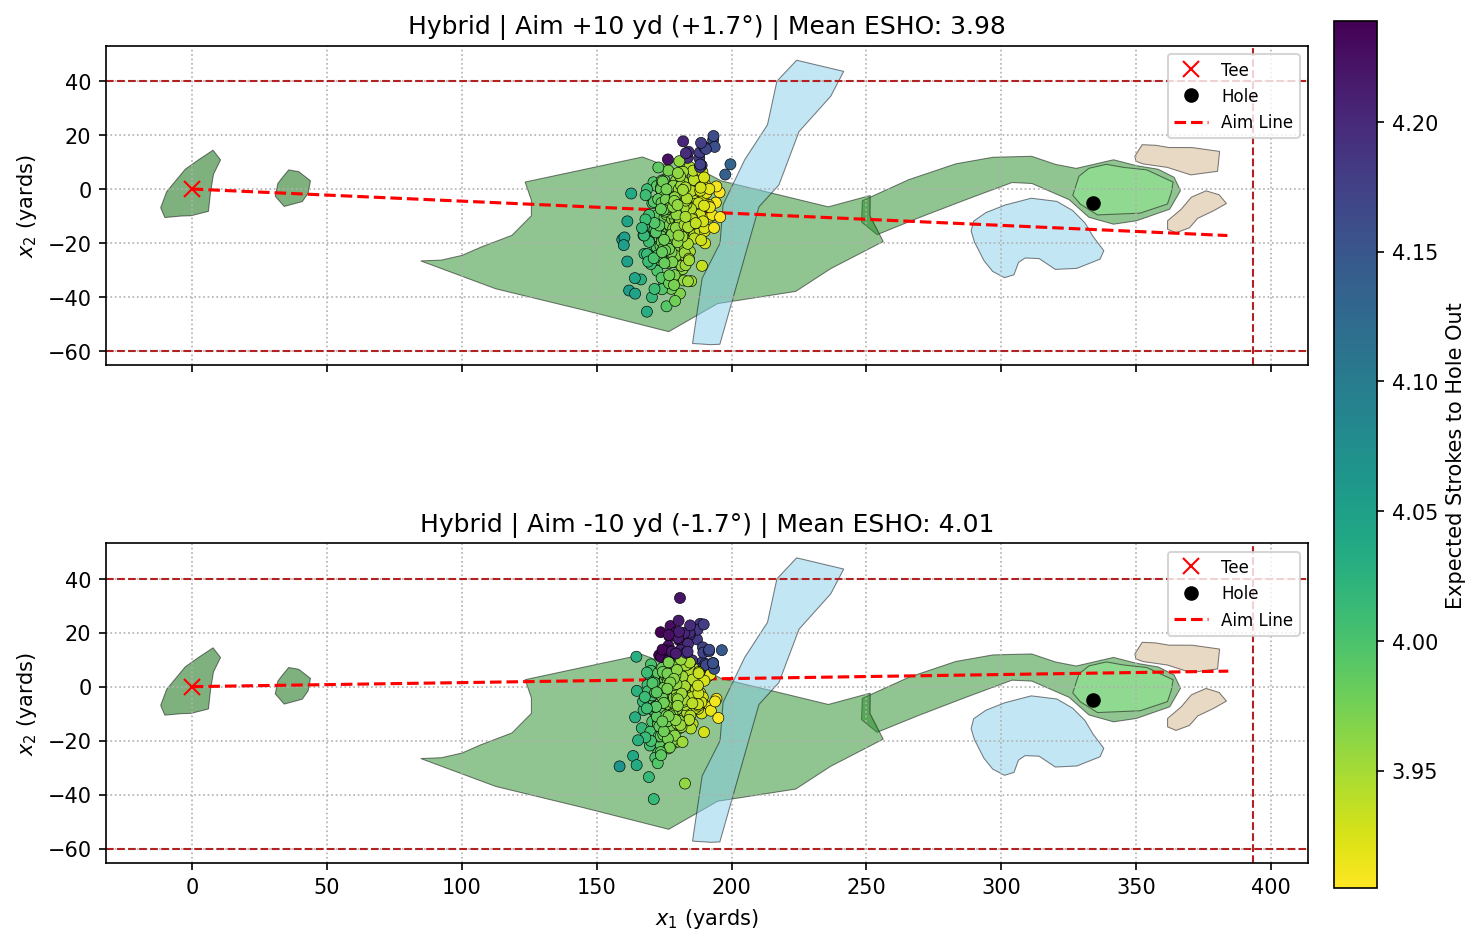
\includegraphics[width=0.75\linewidth]{images/shot_outcomes_stacked.png}
    \caption{Simulated outcomes for a single shot type (Hybrid, $N=300$) at two aimpoints, $\aimpoint=+10$y (top) and $\aimpoint=-10$y (bottom), sharing one colour scale. Each landing is coloured by its expected strokes to hole out, showing how the same dispersion pattern is scored differently depending on where it lands relative to the green, hazards, and the OB boundary.}
    \label{fig:both}
\end{figure}

\subsubsection{Step 3: Minimising Expected Strokes}
\label{subsec: minimise}

We proceed to the optimisation step, which returns the optimal strategy. For a given strategy, defined by a labelled shot type $s$ and aimpoint $\aimpoint$, we have a set of $N$ simulated landing positions $\Samp^{s\aimpoint} = \{\samp^{s1\aimpoint}, \samp^{s2\aimpoint}, \ldots, \samp^{sN\aimpoint}\}$. 

For each simulated shot $i$ (which has a defined $s$ and $\aimpoint$), we evaluate the outcome by querying our $AG(\out)$ (see Eq. \eqref{eq: AG}) at the landing coordinate $\samp^{si\aimpoint} =  \rotation(\aimpoint)\samp^{si} $. The ``cost'' of the shot is the sum of the stroke taken to reach the first point plus the expected strokes required to hole out.

$$\text{Cost}^{si\aimpoint} = 1 + AG(\samp^{si\aimpoint} )$$

We then aggregate the individual outcomes to compute the empirical risk (average expected strokes) for the specific strategic configuration:
\begin{align}
\label{eq: rmu}
    R_\mu(\delta) = R_\mu(s, \aimpoint) = \frac{1}{N} \sum ^N_{i=1} (1+ AG(\samp^{si\aimpoint}))
\end{align}

Equation \eqref{eq: rmu} is computed iteratively across all feasible shots in the player's bag and a discretised range of aimpoints (e.g., $\aimpoint \in [-20, +20]$ in $1^\circ$ increments). The optimal strategy for shot on a specific hole is the pair $(s^*, \aimpoint^*)$ which minimises the risk surface:

$$\delta_{opt} = \arg \min_{s, \aimpoint} R_\mu(s, \aimpoint) = (s^*, \aimpoint^*)$$

We convert the optimal angle $\aimpoint^*$ to yards (left or right of the pin) by using basic trigonometric conversions which make the output actionable for the player. Our three-step process transforms abstract data into concrete recommendations on which the player can then operate.

\subsection{Modeling Chained Decisions. Par 4s \& Recursive Optimisation.} 
\label{subsec: par4}

When considering par 4s, a key insight is that we can treat them mathematically as par 3s featuring a highly variable tee box. Because we have already established a robust Gaussian Process Regression framework for evaluating single-shot approaches to the green (as detailed in Section~\ref{subsec:par3}), we can leverage the existing machinery recursively. We model complex, multi-shot holes through a three-stage process:
(1) pre-computing the optimal approach from a dense grid of all possible fairway positions using our Par 3 logic, (2) anchoring these purely-simulated low-fidelity values to location-specific historical outcomes (high-fidelity data) via a multi-fidelity Gaussian Process, and (3) computing the optimal tee shot evaluated against this fused surface.

\subsubsection{Step 1a: The ``Strategic Blanket'' (Pre-computing Approaches)}
\label{subsec: strategicBlanket}

To connect the player's shot distribution to the continuous course topography, we first need to understand the scoring potential of every intermediate landing zone. We achieve this by evaluating a dense grid $\mathcal{G} = \{\mathbf{g}^1, \mathbf{g}^2, \ldots, \mathbf{g}^M\}$, where $\mathbf{g}^j = (x_1^j, x_2^j)$ of fairway and near-fairway locations ranging from $50$ to $350$ yards from the green. These grid points represent potential second-shot locations.

At this stage, compute the first layer of data: our low-fidelity dataset. We treat each grid point $\mathbf{g}^j$ as a temporary teebox, where we run the exact same Monte Carlo simulation protocol used for Par 3s to capture how player-specific dispersion interacts with local course elements (e.g., water hazards, sand traps):

\begin{enumerate}
    \item Identify the lie at $\grid^j$ - fairway, rough, or bunker --- to select the appropriate shot distribution to sample from the player shot distribution dataset. If $\grid^j$ is on water, simulate dropping with the same logic described in the Equation \eqref{eq: AG}.
    \item Simulate shots for all $s$ and $\theta$ as described in Section \ref{subsec: playerSim} from the temporary ``origin'', $\grid^j$.
    \item Identify the strategy $(s^*, \aimpoint^*)$ that minimises expected strokes said location, $\grid^j$.
    \item Report the minimum risk value (ESHO) $R_{\mu}(s^*, \aimpoint^*)^j$, to use as values in the next phase.
\end{enumerate}

The collection of minimal ESHO values, calculated across the grid $\mathcal{G}$, constitutes our low-fidelity dataset.

The recursive evaluation yields a minimal ESHO value for every point on the grid (\fillin \nts{I need to think about whether i want an image here}). We then fit a secondary Gaussian Process model to these low-fidelity ESHO values across all $\mathbf{g}^j$. This creates a new continuous surface, $f_{approach}^L: \mathbb{R}^2 \to \mathbb{R}^+$, which we term the ``strategic blanket.'' Crucially, when evaluated at a coordinate $\mathbf{x}^l$ on the fairway, $f_{approach}$ does not return a value representing the raw, passive difficulty of the terrain. Rather, it represents the best possible expected score a player can achieve from any given location assuming they play optimally from that point forward.

\nts{here i would reference the low fidelity plot too possibly}

\begin{figure}[t]
    \centering
\includegraphics[width=0.5\linewidth]{images/GPRPar4.png}
    \caption{\textbf{The ``Strategic Blanket'' ($f_{approach}$).} 
    A visualisation of the recursive optimisation step. The heatmap does not represent the difficulty of the hole, but rather the optimal expected score achievable from any given grid point $\mathbf{g}^j$ (50--350 yards), assuming optimal play from that point forward. The ``valleys'' (dark blue) represent ideal landing zones for a tee shot. \nts{probably remove}}
    \label{fig:strategic_blanket}
\end{figure}


\subsubsection{Step 1b: The "Strategic Blanket" (Multi-fidelity Implementation)}

The Gaussian Process fit on the low-fidelity data, $f_L$, is only as accurate as the shot simulation and green/short-game models feeding it --- it has no way to reflect real terrain effects (drainage, compacted rough, a fairway that plays firmer than assumed) it was
never told about. This is precisely the region of the course where both fidelities of data described in Section~\ref{ref:idealData} are actually available: real, location-specific strokes-to-hole-out observations recorded at rough, fairway, sand, and water-adjacent
coordinates within driving distance; historical outcomes from play on the particular hole of interest.

We fuse the two data sources using the \newcite (Kennedy O'Hagan) multi-fidelity model. Conceptually, the fused surface is:
\begin{align}
f_{approach}(x_1,x_2) = \rho \cdot f_{L}(x_1,x_2) + \lambda(x_1,x_2)    
\end{align}

where $\rho$ is a learned scalar correcting the simulation's overall bias, and $\lambda$ is a GP correcting its spatial errors. We implement this a couple of steps.

\begin{enumerate}
    \item \textbf{Fit the simulation GP.} We fit $f_{L}$ (RBF kernel, \texttt{GPyTorch ExactGP}) to the 280 grid points of ESHO values. This gives a posterior mean $\mu_{L}(x_1,x_2)$ at any course location.

    \item \textbf{Fit the discrepancy GP, with the simulation baked into its mean.} We fit a second GP, $\lambda$, directly to the real observed outcomes $y_H$ at their locations $(x_1,x_2)$. Rather than fitting $\lambda$ to residuals computed by hand, we set the GP's \emph{prior mean function} to $\rho \cdot \mu_{L}(x_1,x_2)$:
    $$m(x_1,x_2) = \rho \cdot \mu_{L}(x_1,x_2), \qquad \rho = \text{softplus}(\rho_{raw}) > 0$$
     $\delta$'s kernel still operates only on the physical location $(x_1,x_2)$. This keeps the correction spatially local: two locations correct each other only insofar as they are physically close, matching how real course hazards (a drainage ditch, a patch of heavy rough) are actually localized in space, not in ``simulated difficulty.'' $\rho$ and the kernel hyperparameters are learned jointly via maximum marginal likelihood. Given that $\rho\mu_{L}$ is already inside the GP's mean function, we can then simply evaluate the posterior mean of our new GP.
\end{enumerate}

Where real data is available nearby, $f_{approach}$ pulls toward historical data; away from any historical observation, $\lambda$'s uncertainty widens back to the simulation's own uncertainty, and $f_{approach}$ collapses to $\rho \cdot \mu_{L}$. From this point on, $f_{approach}(x_1,x_2)$ replaces $f_{sim}$ in downstream tee-shot optimisation.



\begin{figure}[h]
    \centering
    \includegraphics[width=\linewidth]{images/multifidelity_diagnostics_real.png}
    \caption{Left: $f_{sim}$, the simulation-only GPR ($\mathcal{D}_L$ alone). Centre: the fitted KOH discrepancy $\delta(x) = f_{fused} - f_{sim}$, with observed strokes overlaid. Right: the fused surface $f_{fused} = \rho \cdot f_{sim} + \delta$, pulling toward $\mathcal{D}_H$ where observations are nearby and collapsing back to $\rho \cdot f_{sim}$ elsewhere.}
    \label{fig:multifidelity_diagnostics}
\end{figure}

\subsubsection{Step 2: Optimising the Tee Shot}
With $f_{approach}(\out)$ acting as our main evaluation function (replacing $AG(\out)$), the par 4 tee shot optimisation becomes mathematically equivalent to the par 3 problem.

We simulate tee shots for long-range clubs (Driver, Woods, and Long Irons) using the player's dispersion parameters $\hat\mu_{s},\hat\Sigma_{s} $, now assuming to be hitting off the tee. For each simulated landing point $\samp^{si\aimpoint}$ (derived from the same Monte Carlo process described in Section \ref{subsec: playerSim}), the cost is no longer derived from the green model, but from our adjusted strategic blanket built upon the multi-fidelity GP:
$$\text{Cost}^{si \aimpoint} = 1 + f_{approach}(\samp^{si\aimpoint})$$
Our optimisation seeks the shot type and aimpoint that lands the ball in the areas of $f_{approach}$ ---areas where the subsequent shot is easiest and therefore the expectation of the optimal choice is lowest - while avoiding the hazards or difficult angles. 

We aggregate the costs once again to find the risk of the tee shot:

$$ R _{\mu_{tee}}(\delta)= R_{\mu_{tee}}(s, \aimpoint) = \frac{1}{N} \sum^N_{i =1} (1 + f_{approach}(\samp^{si\aimpoint}))$$

As such, the optimal tee strategy is defined as:
$$\delta_{opt}  = \arg \min_{s, \aimpoint} R_{\mu_{tee}}(s, \aimpoint) =  (s^*_{tee}, \aimpoint^*_{tee})$$

Our recursive framework allows the model to make nuanced trade-offs, potentially suggesting more conservative options such as hitting the shorter distance club not just to ensure landing on the fairway, but to avoid bringing other trouble into play (water or bunkers).

\begin{figure}[htb]
   \centering
    
    % --- Top Image: Conservative Strategy ---
    \begin{minipage}{\textwidth}  % Increased width for vertical stacking
        \centering
        \includegraphics[width=\linewidth, height=.25\linewidth]{images/ESHOOptimalPar4.png}
        \caption*{(a) Conservative Strategy ($R_\mu$)}
    \end{minipage}
    
    \vspace{0.2cm} % Add vertical space between the two images
    
    % --- Bottom Image: Aggressive Strategy ---
    \begin{minipage}{\textwidth}
        \centering
        \includegraphics[width=\linewidth, height=.3\linewidth]{images/BirdieOddsOptimal.jpg}
        \caption*{(b) Aggressive Strategy ($R_B$)}
    \end{minipage}
    \caption{\textbf{Strategic Divergence based on Loss Function.} 
    (a) When minimising Expected Strokes to Hole Out ($R_\mu$), the model identifies a risk-averse strategy: a 5-wood lay-up short of the water hazard, prioritising variance reduction. The dotted grid acts as a recursive roadmap for the subsequent approach shot: the fill colour of each dot indicates the optimal club selection (as indicated by the legend), while the text label specifies the optimal aimpoint offset in yards (positive values aim right of the pin, negative aim left).
    (b) When maximising Birdie Probability ($R_B$), the model shifts to a high-variance strategy: a Driver aimed over the hazard, accepting the penalty risk in exchange for a higher probability of a short approach shot. While a similar club roadmap as (a) exists for this objective, the heatmap here visualises the computed \textit{likelihood} of securing a birdie from each coordinate, illustrating the high-reward zones that drive this aggressive strategy.}
    \nts{Completely replace these plots}
    \label{fig:strategy_comparison}
\end{figure}

\subsection{Modeling Alternative Loss Functions. Maximisation of Birdie Probabilities.}
\label{subsec: par4b}

Up until now, our optimisation strategy has focused on minimising the expected number of strokes to hole out. This approach naturally produces conservative strategies ---decisions that prioritise avoiding high-penalty disasters (such as hitting the ball into water hazards or out of bounds) over chasing rare, high-reward outcomes. In statistical terms, this conservative play minimises the variance of the score distribution to protect the mean.

However, golfers are often faced with high-tension scenarios where consistency becomes inconsequential. If a player needs a birdie to make the cut, force a playoff, or win a tournament, a par may be functionally equivalent to a double bogey. In these moments, aggressive strategies are required. Here, the player willingly accepts a higher expected score (and higher variance) in exchange for increasing the probability mass in the lower tail of the distribution (i.e., in the case of a par 4, the chance of holing it in 3 or fewer strokes).

To model the change in objective, we alter our loss function by converting the data used to train the GPR and slightly altering one of the GPR fitting steps.



\subsubsection{Step 1: The Probability Surface}
We begin by returning to the raw data generated on the green (as described in Section \ref{subsec: greendata}). In the par 3 and par 4 expectation minimisation models described earlier, each data point collected on a green was a count of strokes (e.g., 1, 2, or 3) from location $\coord$. For our new objective, we perform a binary conversion on the training data outcomes $\mathbf{y}$. 
\[y_{binary} = \begin{cases}
1, & \text{if strokes} \le 1 \;\text{(holed)} \\
0, & \text{if strokes} > 1 \;\text{(missed)}
\end{cases}\]

\textit{Why one-putts?} A player typically makes par by two-putting. So the surest route to a birdie is a one-putt, and the probability of one-putting is what we model.

We place a latent GP $g(\out) \sim \mathcal{GP}(0, k(\out,\out'))$ over the green and link it to the binary outcomes with a Bernoulli likelihood and a probit link:
\[y_i \mid g(\out_i) \sim \text{Bernoulli}(\Phi(g(\out_i)))\]
where $\Phi(\cdot)$ is the standard normal CDF.

Because the probit likelihood is non-Gaussian, we cannot evaluate the posterior in a closed form the way we can for a standard GP. Instead, we approximate it using Stochastic Varational Inference, implemented in \texttt{GPyTorch's} framework (\texttt{ApproximateGP}, \texttt{CholeskyVariationalDistribution}, and \texttt{VariationalStrategy}). The model is optimised using the Evidence Lower Bound, with \texttt{BernoulliLikelihood} uses Gauss-Hermite quadrature to squash the GP's latent predictions into a $[0,1]$ probability.

This gives a continuous Birdie Probability Surface:
\[f_{birdie}(\out) = \Phi(\bar g(\out))\]
the probability of one-putting from coordinate $\out$, where $\bar g(\out)$ is the latent GP's posterior mean. The surface decays sharply with distance: 3 feet from the cup carries real value, 15 feet is close to worthless when a birdie is required. 
\nts{maybe add image}


\subsubsection{Step 2: Recursive Maximisation for Birdie Likelihood Maximisation}
With the birdie probability surface defined over the green, we re-evaluate strategic decisions. We run our recursive simulation framework with a modified evaluation logic aimed at maximising the probability of carding a birdie:

\begin{enumerate}
\item \textbf{Approach Simulation:} For all simulated approach shots $\samp^{si\aimpoint}$ (the rotated samples from the Monte Carlo step in Equation \eqref{eq: shots}), we query the new surface:

\[
\mathbb{P}(\text{Birdie} \mid \mathbf{z}^{si\aimpoint}) = \begin{cases}
    f_{birdie}(\mathbf{z}^{si\aimpoint}) & \text{if } \mathbf{z}^{si\aimpoint} \in \Omega_{green} \\
    0 & \text{else}
\end{cases}
\]

Note that we make the simplifying assumption that shots missing the green ($\samp^{si\theta} \not\in \Omega_{green}$) have negligible probability of being holed for birdie.

\item \textbf{Risk Calculation:} The risk we seek to minimise is the probability of failure (not achieving a birdie or better). We  aggregate the probabilities across all $N$ samples:

$$R_{B}(\delta)= R_{B}(s, \aimpoint) = 1 - \frac{1}{N} \sum_{i=1}^{N} \mathbb{P}(\text{Birdie} \mid \mathbf{z}^{si\aimpoint})$$

\item \textbf{Optimal Aggressive Strategy on Par 3s:} Finally, we identify the strategy that minimises the probability of failure (thereby maximising birdie probability) by iterating over all feasible shots and aim angles:

$$\delta_{opt} = \arg \min_{s, \aimpoint} R_B(s, \aimpoint) = (s^*, \aimpoint^*)$$

$\delta^{opt}$ yields the specific club $s^*$ and aimpoint $\theta^*$ that maximise the odds of acquiring a birdie, ignoring the potential higher variance of the shot.
\end{enumerate}

\subsubsection{Step 3: Aggressive Tee Shots}

For par 4s, we repeat the ``strategic blanket'' process described in Section~\ref{subsec: par4}, but with a fundamental shift in the evaluation metric.

We move away from fitting a multi-fidelity GP on the ESHO of the approach shots, and fit a regular Gaussian Process on the birdie probability values we compute in step 2. That is, a newly fit GP that maps the highest birdie probability achievable from every grid point $\mathbf{g}^j$ on or around the fairway. Said surface, $f_{approach_b}: \mathbb{R}^2 \to [0,1]$, presents the highest values at locations that offer the best statistical chance of converting a birdie on the subsequent shot.

The ``aggresive model'' $f_{approach_b}$ relies strictly on low-fidelity simulated approach outcomes. Because historical tournament data record raw strokes from fairway locations instead of binary ``birdie success'' flags tied to specific prior landing coordinates, high-fidelity birdie data is not accessible to us across the fairway grid. Consequently, for a par 4, $f_{approach_b}$ is constructed as a standard, exact GP trained on the low-fidelity data and does not take into account the idiosyncrasies of the fairway.

When optimising the tee shot, the model aggregates these probabilities to find the strategy that maximises the potential for a birdie. We simulate the tee shots as before, but the cost function is inverted to represent the probability of success:
$$R_{B_{tee}}(s, \aimpoint) = 1 - \frac{1}{N} \sum^N_{i =1} f_{approach_b}(\mathbf{z}^{si\theta})$$
Consequently, the optimal aggressive tee strategy is identified by minimising this risk (failure) function: 
\[\delta_{opt} =\arg\min_{s,\aimpoint} R_{B_{tee}}(s, \aimpoint) = (s^*_{tee}, \aimpoint^*_{tee})\]
After assessing these values at the tee, the golfer would do best to choose the provided $s^*$ and $\theta^*$ for their first shot. \change In our example (Figure \ref{fig:strategy_comparison} (b)) the optimal decision is Driver aimed $+6y$ (aimed $6$ yards right).
The output of the optimisation for birdie can often be drastically different from optimisation for ESHO. Which in some ways, is exactly what we want to see ---different optimal decisions for different objectives. 

\nts{maybe images of different objective outptus}

\subsection{Model Requirements and Outputs}

\subsubsection{A Single Answer?}
\label{subsec:Convergence}

The recommendations our framework produce rest on a choice of $N$, the number of Monte
Carlo samples drawn per candidate decision (Section~\ref{subsec: playerSim}). Too few samples, and a recommended club or aimpoint may simply reflect simulation noise rather than a genuine difference in expected cost; too many samples, and computation is spent recalculating outcomes that would not have changed the recommendation, regardless. In order to determine the computational cost and requirements of our model --- specifically, how large $N$ needs to be before a strategy recommendation can be trusted, and what that stability costs in practice -- we studied how the
model's output at each grid point changes as $N$ grows, across a large number of independent
simulation seeds.

Instead of simulating from scratch at each sample size, we accumulated shots: we let $N$ start at $10$ and grow in steps of 10 up to a ceiling of $N_{max}$. After each increment, the full $M = 280$-point optimal snapshot over $\mathcal{G}$ (Section~\ref{subsec: par4}) \nts{add equation} is recomputed, and a stopping rule declares the search converged once $k = 3$ consecutive snapshots are identical. The full sweep ($N= 10, 20, \ldots, 300$) was repeated for 100 independent seeds, each producing different Monte Carlo simulations on each of the grid points and club-aimpoint combination.


Two convergence metrics were tracked: 
\begin{enumerate}
    \item \textit{Sequential match rate:} for each seed, a grid point ``matches'' between consecutive snapshots ($N$ and $N+10$) if the recommended club is unchanged and the recommended aimpoint changes by no more than a tolerance ($\pm 2^\circ$ between snapshots and $\pm3^\circ$ \nts{i probably want to change this. yards is better.} between seeds), with the percentage of matching points across all $M = 280$ tracked as a function of $N$ and averaged across seeds.
    \item \textit{Cross-seed agreement:} at each $(\mathbf{g}^j, N)$, the fraction of the 100 seeds whose recommended club matches across identical grid points.
\end{enumerate}

Using the aforementioned player profile on the par 4, at approximately $N \approx 180$ shots per grid point, the mean sequential match rate was around 80\%. As $N$ increased, closer to $N = 300$, the match rate narrowly clustered at 87-91\% across seeds never reaching 100\% at the $N = 300$ ceiling. When looking at $N = 300$, 35 of the 280 grid points fail to show cross-seed agreement, concentrated in a band around $y \approx 100$ yards, corresponding to a distance that presents many possible suitable club options. The $80-120$ yard band converges worst, opposite of our original hypothesis that longer approach shots (clubs with larger dispersion) would be the hardest to resolve. Along with these antithetical results we see that the $50-80$ yard wedge range also converges early. 

Upon further inspection, we realise that the points that never converge don't seem to drift toward a single answer as $N$ grows, instead, they oscillate between multiple combination candidates, whose expected strokes are, in fact, statistically tied. We come to the conclusion that the convergence plateau isn't a symptom of insufficient sampling; but rather a direct consequence of the fact that there are near-identical options at these locations, whose expectation doesn't vary significantly from a clear optimal. Our observations motivate Section \ref{subsec:Options}.



\subsubsection{Near-ties and One-standard-error Decision Sets}
\label{subsec:Options}

The convergence plateau in Section \ref{subsec:Convergence} suggests that a subset of grid points never converge because two or more $\comb$ strategies are statistically indistinguishable given the simulated outcome variance. We test this directly by comparing each grid point's simulated outcome distributions against their own sampling uncertainty, using the standard error of the mean,
\begin{align}
    SE(\delta) = \sqrt{\sigma^2(\delta)/N}
\end{align}
where $\sigma^2(\delta)$ is the empirical variance of the simulated ESHO outcomes for a given decision $\delta$, at a given location $\coord$. Rather that reporting a single optimal combination, we define a equivalence set,
\begin{align}
    \mathcal{E}^* = \left\{ \comb : R(\comb) \leq R_{\min} + e \cdot SE(s, \theta)_ {\min}) \right\}
\end{align}
here $\comb_{\min}$ is the ``optimal'' combination. We set $e = 1$.  Rather than a single prescription, the model hands the player a ranked shortlist of statistically equivalent strategies instead of a singular choice. \nts{maybe expand}

\nts{heatmap with multiple combinations plot }

\nts{I want to re-run convergence and see if the entire strategy grid remains statisticall indistinguishable from the rest no matter how $N$ is increased and when that happens.}

\subsection{Generalised Observations}
\label{subsec: genObs}
Section \ref{sec: Intro} noted Broadie's empirical finding drawn from observed PGA Tour outcomes, that distance is the strongest predictor of scoring success. We assessed the same question directly within our simulation framework, choosing to contrast the difference in expected outcome when changing a player's average distance versus consistency. We took our baseline player profile and systematically varied two independently controllable player parameters: average distance per shot and their accuracy. We ran our model implementing 81-configurations, controlling: distance shift, $\alpha \in \{-9, -6, -3, 0, 3, 6, 9, 12, 15\}$ yards applied as an additive shift to every club's mean carry distance; and a dispersion scale, $\beta \in \{0.80, 0.85, 0.90, 0.94, 0.97, 1.00, 1.03, 1.06, 1.09\}$, applied as a multiplicative scaling of every club's full shot covariance matrix. Pairing all of the possible combinations allowed us to evaluate: distance with dispersion held at baseline; dispersion varying with distance held at the baseline; and both varying jointly. 

Each of the 81 configurations was simulated on the same $M = 280$ strategy grid with $N = 300$, fitting the second-stage GP on the best ranked combinations (ignoring equivalent combinations), to evaluate the optimal tee-shot placements under said configurations. 

\nts{equivalent outcomes plot }
\begin{figure}[h]
    \centering
    \includegraphics[width=0.5\linewidth]{images/missing images/holeoutline_sensitivity_dist0.00_disp1.0000.png}
    \caption{Baseline configuration ($\alpha=0$, $\beta=1.00$) equivalence-set heatmap with the hole outline overlaid.}
    \label{fig:holeoutline_sensitivity}
\end{figure}

\nts{Complete results and discussion. Should sensitivity go here or in results?
maybe plot with arrows - what does that say?}

\section{Results}
\label{sec:Results}
The primary objective of our work was to establish a computationally grounded methodology for converting individual player performance data into actionable strategic recommendations by employing Gaussian Process Regression. Ultimately, we wanted to demonstrate that we could generate actionable strategic recommendations based on varying player objectives. Our simulation results confirm that our model effectively learns course-specific risk surfaces and adapts its recommendations accordingly. 

\subsection{Risk Surface Generation}
The GPR model successfully learns continuous risk surfaces from discrete, noisy data points. For the par 3 case study (hole 9, Mountain Meadows), the model generated a smooth Expected Strokes to Hole Out (ESHO) surface that accurately reflected the penalty structure of the hole. The surface naturally exhibited higher ``risk'' values near the water hazard and bunkers, and lower values in the wider part of the green, effectively interpolating difficulty in unobserved regions. Our model subsequently gave us a very reasonable recommendation.

\subsection{Strategic Divergence: Conservative vs. Aggressive}
One of the most valuable finding is the clear divergence in optimal strategy when switching between loss functions (minimising expected strokes versus maximising birdie probability), visualised in Figure \ref{fig:strategy_comparison}.

\begin{itemize}
    \item \textbf{Minimising Expected Strokes (Conservative):} When minimising $R_\mu(\delta)$, the model recommends strategies that prioritise variance reduction. On the par 4 simulation, the ``Strategic Blanket'' identified that the optimal tee shot was not necessarily the driver. Instead, our model suggested hitting a 5-wood (a safe choice off the tee) aimed at the widest part of the fairway, sacrificing distance to avoid the high-penalty zone (the water penalty crossing the hole) that the driver's wider dispersion would bring into play. 
    
    \item \textbf{Maximising Birdie Probability (Aggressive):} Conversely, when minimising $R_B(\delta)$, the model shifted to a high-variance, high-reward approach. The model recommends a more aggressive approach by hitting the driver over the water and accepting a non-zero probability of a penalty in exchange for substantially shorter approach shot, which would intuitively have a smaller dispersion.
\end{itemize}

In summary, the framework works as intended: it does not simply output a single ``best'' shot, but effectively quantifies the trade-offs between consistency and scoring potential, providing players with a roadmap that they can implement regardless of the outcome of their first shot.

\section{Discussion}
\label{sec:Discussion}

\nts{add that our work is a pre-cursor which roll-out and vertical trajectory can extend}
Our project serves as a proof-of-concept for the derivation of mathematically reasonable golf strategies under a Bayesian paradigm. By treating the course as a continuous probabilistic surface, we accept the variability and uncertainty behind a shot, directly modeling it. As outlined earlier, our approach works; however, several limitations must be addressed before the framework can be deployed widely.

Perhaps the most important of our limitations is the simplification of our ball flight physics. Our model currently assumes that the ball stops at its carry distance, when in reality shots usually have roll-out. How much a ball rolls out is complicated to compute as it depends on landing angle, spin rate, and ground firmness. On hard fairways or greens a ball may roll-out 20-40 yards, potentially bringing hazards into play that we deemed unreachable in our statistical analysis based on carry distance alone. Furthermore, we do not model the vertical trajectory (apex height) or shot shape (draw/fade), meaning the model cannot currently account for obstacles that require clearance, such as tall trees.

The current iteration of our project also assumes a static environment. We ignore meteorological conditions such as wind speed, direction, temperature, and air density, all of which drastically affect carry distances. While these variables can be parametrised, implementing variables that can change quickly during a tournament presents a formidable challenge. Additionally, our model assumes a constant green speed and ignores elevation changes from tee to green, which are critical for accurate club selection.

While our green putting model is robust, the ``around-the-green'' data used in our analysis relies on sparse interpolated averages from historical PGA Tour baselines rather than player-specific data. This assumes the player possesses ``average'' professional scrambling ability, which may mask individual weaknesses (e.g., a player who is statistically poor from sand bunkers should be advised to avoid them more aggressively than our model currently suggests).

Our project also presents unique opportunities. A distinct advantage of GPR is the generation of posterior variance estimates, which quantify the model's uncertainty. Future iterations should explicitly incorporate these interval estimates into the strategy recommendation engine. By distinguishing between high-confidence predictions (where data is dense) and regions of high uncertainty (where data is sparse), future models could differentiate between strategies that are genuinely ``safe'' and those that merely appear optimal because the model lacks sufficient data on local hazards.

Similarly, we would like to extend our framework to model par 5 holes which introduce the consideration of three chained shots in a row. Additionally, testing the model on diverse course styles ranging from links-courses (firm course with high roll and few hazards) to target golf (courses with many obstacles that force the player to fly the ball past them) would validate the robustness of our proposed framework.

Currently, the model utilizes a proxy ``average LPGA'' profile. Future work involves ingesting real shot data from distinct populations (e.g., elite male amateurs vs. seniors vs. collegiate athletes) to observe how optimal risk surfaces change based on power and consistency disparities.

Ultimately, this project lays the mathematical groundwork for a ``digital caddie'' evolving with the player by turning every shot recorded into a smarter decision for the future.

\appendix
\section{Data Generation Methodology}
\label{sec:Appendix}
In the absence of granular, shot-level tournament data (such as PGA Tour ShotLink data) and player-specific data, we developed a robust synthetic data generation pipeline to construct realistic two-dimensional scoring distributions by combining course digitisation, empirical statistical interpolation, and probabilistic simulation.

We constructed a proxy player profile representing an ``average'' LPGA Tour player using publicly available launch monitor data \parencite{trackman2024averages}.

\subsection{Course Geometry and Lie Classification}
\label{app: course-representation}

To create a spatially accurate environment for our model, we digitised the layout of hole 9 at Mountain Meadows Golf Course in Pomona, California.
\begin{enumerate}
    \item \textbf{Vector Mapping:} The course layout was initially scraped using OpenStreetMap \parencite{openstreetmap} and imported into QGIS \parencite{qgis} for refinement.
    \item \textbf{Polygon Classification:} Features were exported as WKT (Well-Known Text) polygons, allowing for the discrete classification of any coordinate $\coord$ into specific lie types (Fairway, Rough, Bunker, Green, or Water) using the \texttt{Shapely} library in Python \parencite{shapely}. This geometric classification is the foundational layer for all subsequent scoring evaluations.
\end{enumerate}

\subsection{Green Surface Data Generation}
\label{app: green-surface data}
To model putting difficulty beyond simple distance estimates, we constructed a multivariate dataset that accounted stroke differences across the complex topography of a green. This process involved a multi-stage pipeline designed to transform univariate averages into spatially aware discrete outcomes, creating data that would be more representative of that collected at an actual tournament.

\begin{enumerate}
    \item \textbf{Surface Topographical Modeling.} We defined a continuous height function $z(x_1, x_2)$ to simulate a realistic putting surface featuring a general tilt, undulating bumps, and a mid-green tier. By defining a height function, we were then able to calculate slope vectors and break severity at any point on the green.
    \item \textbf{Baseline Interpolation with Noise.} We first interpolated baseline average putts values from Mark Broadie's empirical estimates in Table \ref{tab: ESHO_Putts}. 
    To mimic real-world heteroscedasticity (where variance increases with distance) and data sparsity at long range, we generated noisy synthetic samples centred  at Broadie's empirical means.
\[ y_{sample} \sim \mathcal{N}(f_{Broadie}(d), \sigma_d^2) \]
We then fit an intermediate GPR model to the synthetic samples, creating a smooth, continuous interpolator capable of generating posterior predictive distributions of ESHO for any distance $d$. The Gaussian Process also captured both the mean trend and the increasing uncertainty at longer ranges.
\begin{table}[h!]
    \centering
    \scriptsize
    \caption{\textbf{PGA Tour Putting Statistics by Distance.} The ``Average putts'' column represents the PGA Tour putting benchmark used in strokes gained computations. The values are based on an analysis of nearly four million putts on the PGA Tour from 2003 to 2012, as detailed in \parencite{Broadie_2014a}.}
    \label{tab: ESHO_Putts}
    \renewcommand{\arraystretch}{1.2}
    \begin{tabular}{l|*{9}{c}}
        \toprule
        \textbf{Distance (feet)} & 2 & 3 & 4 & 5 & 6 & 7 & 8 & 9 & 10 \\
        \midrule
        \textbf{One-putt probability} & 99\% & 96\% & 88\% & 77\% & 66\% & 58\% & 50\% & 45\% & 40\% \\
        \textbf{Three-putt probability} & 0.0\% & 0.1\% & 0.3\% & 0.4\% & 0.4\% & 0.5\% & 0.6\% & 0.7\% & 0.7\% \\
        \textbf{Average putts} & 1.01 & 1.04 & 1.13 & 1.23 & 1.34 & 1.42 & 1.50 & 1.56 & 1.61 \\
        \bottomrule
    \end{tabular}
    
    \vspace{0.2cm} 

    \begin{tabular}{l|*{7}{c}}
        \toprule
        \textbf{Distance (feet)} & 15 & 20 & 30 & 40 & 50 & 60 & 90  \\
        \midrule
        \textbf{One-putt probability} & 23\% & 15\% & 7\% & 4\% & 3\% & 2\% & 1\%   \\
        \textbf{Three-putt probability} & 1.3\% & 2.2\% & 5.0\% & 10.0\% & 17.0\% & 23.0\% & 41.0\%  \\
        \textbf{Average putts} & 1.78 & 1.87 & 1.98 & 2.06 & 2.14 & 2.21 & 2.40  \\
        \bottomrule
    \end{tabular}
\end{table}

\item \textbf{Difficulty Multipliers}
To account for the non-linear difficulty introduced by the green's shape, we computed difficulty multipliers based on the local topography. We evaluated the gradient of the surface at four critical points along the putt's trajectory (50\%, 70\%, 85\%, and 95\% of the distance to the hole) to capture the relevant slope and break.

\begin{itemize}
    \item \textbf{Fall Line Slope:} Penalising downhill putts (where the ball picks up speed) more heavily than uphill ones.
    \item \textbf{Tier Difference:} Adding a strong penalty if the ball and hole are located on different tiers.
    \item \textbf{Side Slope:} Calculating the perpendicular slope at different points of the putt's path to account for large amounts of break.
\end{itemize}

The specific multipliers (provided in Table \ref{tab:multipliers}) were estimated heuristically based on domain expertise, as empirical data for slope-specific putting difficulty is not publicly available. The multipliers adjust the baseline ESHO ($\mu_{base}$) to form an adjusted mean $\mu_{adj}$:
\[ \mu_{adj} = \mu_{base} \times M_{tier} \times M_{side} \times M_{slope} \]

\begin{table}[h!]
    \centering
    \scriptsize
    \caption{\textbf{Topographical Difficulty Multipliers.} Multipliers are applied to the baseline expected strokes to hole out (ESHO) to account for green complexity. \textit{Note: These values are heuristic estimates derived from domain knowledge.}}
    \label{tab:multipliers}
    \renewcommand{\arraystretch}{1.2}
    \begin{tabular}{llc}
        \toprule
        \textbf{Factor} & \textbf{Condition} & \textbf{Multiplier Range} \\
        \midrule
        \textbf{Tier Difference} & No Tier (Diff $< 0.15$) & $1.00$ \\
        (Height diff. between ball \& hole) & Level 1 (Diff $0.15 - 0.45$) & $1.05 - 1.07$ \\
        & Level 2 (Diff $0.45 - 0.70$) & $1.08 - 1.12$ \\
        & Level 3 (Diff $0.70 - 1.00$) & $1.12 - 1.17$ \\
        & Level 4 (Diff $1.00 - 2.00$) & $1.18 - 1.25$ \\
        & Level 5 (Diff $> 2.00$) & $1.40$ \\
        \midrule
        \textbf{Side Slope} & Negligible ($< 0.5\%$) & $1.00$ \\
        (Max perpendicular slope) & Mild ($0.5 - 1.0\%$) & $1.00 - 1.03$ \\
        & Moderate ($1.0 - 2.0\%$) & $1.04 - 1.09$ \\
        & Severe ($2.0 - 3.0\%$) & $1.10 - 1.20$ \\
        & Extreme ($3.0 - 4.0\%$) & $1.20 - 1.25$ \\
        & Unplayable ($> 4.0\%$) & $1.35$ \\
        \midrule
        \textbf{Uphill / Downhill} & Flat & $1.00$ \\
        (Max parallel slope) & Uphill (Mild to Steep) & $1.03 - 1.10$ \\
        & Downhill (Mild) & $1.01 - 1.07$ \\
        & Downhill (Steep) & $1.10 - 1.45$ \\
        & Downhill (Extreme $>3\%$) & $1.45 - 1.60$ \\
        \bottomrule
    \end{tabular}
\end{table}


\item\textbf{Generating Discrete Outcomes}

To generate the final discrete stroke counts used for modeling we executed a probabilistic simulation process that transforms continuous difficulty estimates into discrete scoring distributions:
\begin{enumerate}
    \item \textbf{Sampling and Evaluation:} We selected random $\coord$ coordinates on the digitized green surface. For each point, we computed the Euclidean distance to the hole and queried the intermediate GPR (from Step 2, Appendix \ref{app: green-surface data}) to obtain the posterior distribution of ESHO at that distance. We then applied the topographical multipliers (from Step 3, Appendix \ref{app: green-surface data}) to this distribution, shifting the mean to reflect the specific difficulty of the putt's slope and break.

    \item \textbf{Base Probability Retrieval:} Simultaneously, we retrieved the baseline probabilities $p_1, p_2, p_{3+}$ for holing out in 1, 2, or 3+ strokes from Broadie's empirical Table \ref{tab: ESHO_Putts}, based solely on the Euclidean distance to the hole.

    \item \textbf{Probability Mass Redistribution:} We utilised the shifted ESHO from the GPR to adjust the baseline probabilities. Rather than simply rounding a continuous mean, we redistributed probability mass between discrete outcomes. For example, in locations with high difficulty multipliers (e.g., steep downhill slopes or cross-tier putts), probability mass was shifted from $p_1$ to $p_2$ and to $p_{3+}$, decreasing the likelihood of a one-putt while increasing the risk of a three-putt. This shift was calibrated to ensure the resulting expected value matched our adjusted ESHO ($\mu_{adj}$) while preserving the internal logic of discrete golf scoring.

    \item \textbf{Sampling and Optimization:} We sampled final discrete scores using a discrete inverse transformation on the adjusted probability vectors. Crucially, our framework allowed us to directly extract the probability of a one-putt, $P(\text{Score}=1 \mid x, y)$, from any location, and to fit the GPR in Section \ref{subsec: par4} to data that emulated the ideal data we would collect in a tournament described in Section \ref{ref:idealData}. 
\end{enumerate}
\end{enumerate}

\subsection{Short Game Data Generation}
\label{app: short-game data}

For shots not on the green, we employ a direct interpolation method. Since slope is less critical for these shots than the lie condition, we estimate the expected strokes to hole out (ESHO) by interpolating directly from historical PGA Tour averages based on the distance to the hole and the specific lie type (Fairway, Rough, or Sand). Table \ref{tab:broadie_shortgame} displays the baseline values used for the interpolation, once again derived from Broadie's work \parencite{Broadie_2014a}.

\begin{table}[h!]
    \centering
    \scriptsize
    \caption{\textbf{Average Shots to Hole Out by Lie and Distance.} Values represent the expected number of strokes to hole out from specific distances and lies, derived from PGA Tour ShotLink data (2003-2012) \parencite{Broadie_2014a}.}
    \label{tab:broadie_shortgame}
    \renewcommand{\arraystretch}{1.2}
    \begin{tabular}{cccc}
        \toprule
        \textbf{Distance} & \textbf{Fairway} & \textbf{Rough} & \textbf{Sand} \\
        \textbf{(yards)} & \textbf{(avg shots)} & \textbf{(avg shots)} & \textbf{(avg shots)} \\
        \midrule
        20 & 2.40 & 2.59 & 2.53 \\
        40 & 2.60 & 2.78 & 2.82 \\
        60 & 2.70 & 2.91 & 3.15 \\
        80 & 2.75 & 2.96 & 3.24 \\
        \bottomrule
    \end{tabular}
\end{table}

\subsubsection{Simulating Player-Specific Data}
\label{app: player-data}
We constructed a proxy player profile representing an ``average'' right-handed LPGA Tour player using a simulation based on publicly available carry distance averages \parencite{trackman2024averages}.
\begin{enumerate}\item 
\textbf{Base Averages:} We defined average carry distances for 20 distinct shot types, ranging from a Driver ($223$ yards) to a $60^{\circ}$ wedge ($78$ yards) based off of official data; also including partial wedge shots to bridge yardage gaps for the shorter distances (e.g., a $3/4$ 60-degree wedge). 
\item \textbf{Dispersion Scaling:} To model the natural increase in variance with shot length, we scaled the standard deviations for lateral error ($\sigma_{side}$) and distance error ($\sigma_{dist}$) linearly with carry distance, setting $\sigma_{side} \approx 0.08 \times \text{Avg. Carry}$ and $\sigma_{dist} \approx 0.04 \times \text{Avg. Carry}$. 
\item \textbf{Directional Bias:} We introduced a correlation between lateral miss and carry distance to mimic real ball flight physics. Shots missing left (simulating pulls) were modelled with a positive distance bias ($+5$ yards on average), while shots missing right (simulating fades or pushes) were modelled with a negative distance bias ($-2$ yards on average), this adjustment was heuristically based on domain expertise, as empirical data for these distributions is not publicly available.

\item \textbf{Sampling:} For each club, we generated $N=30$ synthetic shot outcomes by sampling from the resulting bivariate Gaussian distributions, creating the dataset used to fit the player's statistical profiles.
\end{enumerate}

\subsection{Long Game Data Generation}
\label{app: long-game data}
\nts{complete}


\section{Glossary of Terms}
\label{sec:Appendix2}

\begin{itemize}[noitemsep]
    \item \textbf{Lie:} The ground condition or surface where a ball rests. Common lies include:
    \begin{itemize}[noitemsep]
        \item\textit{Fairway}: Closely mown grass offering the standard hitting surface.
        \item\textit{Rough}: Longer grass bordering fairway lies, thicker and more unpredictable.
        \item\textit{Sand/bunker}: Obstacle or hazard filled with sand.
        \item\textit{Green}: Short grass area around the hole used for putting.
    \end{itemize}
    \item\textbf{Club:} Instrument used to hit golf balls. Clubs vary in loft and length, affecting distance and shot shape. Examples used in this paper include: 5-iron, Wood or Driver.
    \item\textbf{Tee/Tee box:} Designated starting area for each hole.
    \item\textbf{Pin/Flag:} The flagstick marking the hole's location on the green.
    \item\textbf{Hazard:} Course obstacles like water or sand bunkers that penalise errant shots.
    \item\textbf{Drop:} Placing the ball back in play after it lands in a water hazard, typically incurring a penalty stroke.
    \item \textbf{Par:} The expected number of strokes a skilled golfer should take to complete a hole. A par-3 hole expects a golfer to finish in 3 shots.
    \item \textbf{Birdie:} The score that is one stroke under par on a hole.
    \item \textbf{Bogey:} The score that is one stroke over par on a hole.
    \item\textbf{Stroke:} A single swing attempt at the ball.
    \item\textbf{Stock shot:} A player's standard, repeatable ``full swing'' given a club.
    \item\textbf{Approach shot:} A shot intended to reach the green, or ``approach'' the pin.
    \item \textbf{Carry distance:} The distance a ball travels through the air before it first touches the ground.
    \item \textbf{Dispersion:} The spread of a player’s shots around their intended target, variable depending on golf club difficulty and individual golfer's tendencies.
    \item \textbf{Aimpoint:} Directional target chosen by the player, defining the centre of their shot dispersion.
    \item \textbf{Short game:} Shots played close to the green (chipping, pitching, putting).
    \item \textbf{Break:} The curve a putt takes due to green slope.
    \item \textbf{Trackman:} A radar launch monitor system that captures detailed shot data, including launch angle, ball speed, spin, and dispersion.
    \item \textbf{ShotLink:} The PGA Tour's proprietary real-time scoring system that captures 3-dimensional coordinates for every shot taken during a tournament.
    \item \textbf{Strokes Gained (SG):} A statistical metric that compares a player's performance against a baseline (typically the PGA Tour average) to quantify the quality of a shot.
    \item \textbf{Smash Factor:} The ratio of ball speed to clubhead speed, used as a measure of energy transfer efficiency.
    \item \textbf{WAGR:} World Amateur Golf Ranking.
\end{itemize}











% -------------------------------------------------------
% END MATTER
% -------------------------------------------------------
\newpage 



\printbibliography[title={References}]

\vspace{2cm}


\section*{Generative AI Statement}
\noindent
During the preparation of this work, we employed generative AI tools to expedite the software development process. ChatGPT (models GPT-4o and GPT-4.1) was used to identify necessary software libraries, outline implementation steps for the coding framework, and assist with debugging. Google Gemini was used to assist in refining some sentence structure and improving the conciseness of some prose. Grammarly was employed for standard grammatical review. These tools served strictly as technical aids for code implementation and language refinement; the conceptual modeling, mathematical logic, and strategic analysis remain as  original intellectual work.

\end{document}
